% version 1.00, date 22/02/16, auteur Matthieu Martins-Baltar
\documentclass[asi]{picInsa}

%Pour le schéma d'architecture
\usepackage{etex}
\usepackage{tikz}
\usetikzlibrary{shapes,arrows,chains}
%FIN Pour le shéma d'architecture


\DeclareGraphicsRule{*}{pdf}{*}{}
\usepackage{pdfpages}

%\usepackage{colortbl}
\usepackage{fancyhdr}
\usepackage{listings} 
\usepackage{mathrsfs}
\usepackage{url}
\usepackage{lmodern}
\usepackage{color}
\usepackage{xcolor}
\usepackage{wrapfig}
\usepackage{graphicx}
\usepackage{pdflscape}
\usepackage{longtable}
\usepackage{sectsty}
\usepackage{lastpage}
\usepackage{multirow}
\usepackage{float}
\usepackage{eso-pic}
\usepackage[french]{minitoc}
\usepackage[babel=true]{csquotes}
\usepackage{tikz}
\addto\captionsfrench{\def\tablename{Tableau}}
\usepackage{vocabulaireUnipik}
%\usepackage{../../ressources/Unipik/vocabulaire/vocabulaireEastpic}

\setcounter{secnumdepth}{4}
\setcounter{tocdepth}{4}
\newcommand{\ligneMaj}[3] {
	\rowcolor[gray]{0.55} \textbf{\textit{#1}} & #2  &  #3\\
	\hline
}
\newcommand{\ligneSup}[3] {
	\rowcolor[gray]{0.65} |\textunderscore \textbf{\textit{#1}} & #2  &  #3\\
	\hline
}
\newcommand{\ligneMed}[3] {
	\rowcolor[gray]{0.75} \hspace{0.25cm} |\textunderscore #1  & #2 & #3 \\
	\hline
}
\newcommand{\ligneSub}[3] {
	\rowcolor[gray]{0.85}  \hspace{0.5cm} |\textunderscore #1 & #2 & #3\\
	\hline
}
\newcommand{\ligneSubSub}[3] {
	\rowcolor[gray]{0.95}  \hspace{0.75cm} |\textunderscore #1 & #2 & #3\\
	\hline
}
\newcommand{\ligneTache}[3] {
	\hspace{1.00cm} |\textunderscore #1 & #2 & #3\\
	\hline
}
\title{\DSI{}}
\author{\Sergi} %à changer


\titreGeneral{\DSI}
\sousTitreGeneral{\nomEquipe}
\titreAcronyme{\DSICourt}
\version{V1.00}
\titreDetaille{\DSICourt\_S\_\nomEquipe\_\versionPrive}
\referenceVersion{\DSICourt\_S\_\nomEquipe\_\versionPrive}
\auteurs{\Matthieu{} \& \Kafui{} \& \Melissa{} \& \Sergi{} \& \Michel{} \& \Julie{} \& \Florian \& \Mathieu}
\destinataires{}%\nomApprobateur{}, \nomTuteurQualite, \nomEquipe, \nomPIC{}}
\resume{Le présent document contient la présentation du \DSE{} \nomEquipe.}
\motsCles{\DSICourt{}}
\natureDerniereModification{ }
\modeDiffusionControle{}

\begin{document}

\couverture{}

 \informationsGenerales{}
% version 1.00, date 20/02/16, auteur Michel Cressant
\begin{pagesService}
	\begin{historique}
		% nouvelles versions à rajouter AU-DESSUS en recopiant les lignes suivantes et en les modifiant :
		\unHistorique{1.00}{21/02/2016}{\Matthieu{} \newline \Kafui{} \newline \Melissa{} \newline \Sergi{} \newline \Michel{}}{Création}{Toutes}

	\end{historique}

        \begin{suiviDiffusions}

            % On place ici les diffusions
        	\unSuivi{1.00}{}{\nomEquipe{}, \nomPIC{}}
          
          
        \end{suiviDiffusions}

%%Signataires
        \begin{signatures}
	   \uneSignature{Vérificateur}{\RQ{},\newline \CPA}{\Pierre{}}{22/02/2016}{pgpic}
       \uneSignature{Validateur}{\CP{}}{\Sergi}{23/02/2016}{pgpic}
	   \uneSignature{Approbateur}{Le client}{\nomClient}{}{}
        \end{signatures}
	
	

	
	
\end{pagesService}



\tableofcontents

\setcounter{chapter}{0}


\chapter*{Introduction}
\label{intro}
% version 1.01 Date 24/03/2016	Auteur Mathieu Medici

\section*{Objet}
L'objectif de ce document est de présenter les principes et les procédures nécessaires à la mise en œuvre de la gestion des configurations prévue par la norme \isoNeufMilleUn.

\section*{Définition}

Le présent document établit les règles et la structure de la gestion des configurations qui doivent être suivies pendant toute la durée du \picCourt. Il contient :
\begin{itemize}
\item les règles de nommage;
\item la description des différents référentiels;
\item les règles spécifiques de \nomEquipe{};
\item la description de l'administration des configurations;
\item la description de la maîtrise des documents;
\item la description de la maîtrise des enregistrements;
\item les règles d'archivage.
\end{itemize}



\chapter{Architecture}
\label{architecture}
% version 1.01, date 23/02/16, auteur Matthieu Martins-Baltar
Cette partie a pour but de décrire l'architecture globale de l'application.\\

L'architecture du projet est une architecture trois tiers, l'utilisateur accède à l'application avec un navigateur web, qui communique avec un serveur distant qui hébergera la partie serveur de notre application (backend), cette application pourra interroger une base de données qui se trouvera possiblement sur un serveur séparé.\\

De plus, l'application serveur sera structurée selon le modèle MVC (figure \ref{MVC}), c'est-à-dire qu'elle s'orientera autour de trois couches qui sont : les vues, les contrôleurs et le modèle. Le rôle du modèle est de faire le lien avec la base de données et de représenter l'ensemble des données selon le modèle du domaine produit en phase de spécification. Les vues ont pour but de représenter la partie interface homme-machine. Enfin, les contrôleurs permettent de faire le lien entre les actions menés dans la vue et la logique métier des modèles. Cette architecture est décrite figure \ref{archi_schema}.


\begin{figure}[!h]
	\begin{center}
	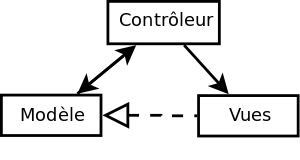
\includegraphics[scale=0.3]{images/MVC}
	\caption{\label{MVC} Patron de conception MVC}
	\end{center}
\end{figure}

\begin{figure}[!h]
	\begin{center}
	%% version 1.00, date 22/02/16, auteur Matthieu Martins-Baltar
% =================================================
% Set up a few colours
\colorlet{lcfree}{Gray}
\colorlet{lcnorm}{Gray}
\colorlet{lccong}{Gray}
\colorlet{lcinput}{Green}
\colorlet{lcoutput}{Red}
\colorlet{lcprero}{Blue}
\colorlet{lcpostro}{Purple}
\colorlet{lcforward}{Orange}
% -------------------------------------------------
% Set up a new layer for the debugging marks, and make sure it is on
% top
\pgfdeclarelayer{marx}
\pgfsetlayers{background,main,marx}
% A macro for marking coordinates (specific to the coordinate naming
% scheme used here). Swap the following 2 definitions to deactivate
% marks.
%\providecommand{\cmark}[2][]{%
%   \begin{pgfonlayer}{marx}
%   \node [nmark] at (c#2#1) {#2};
%  \end{pgfonlayer}{marx}
%  } 
\providecommand{\cmark}[2][]{\relax} 
% -------------------------------------------------

\begin{tikzpicture}[%
	auto,
    >=triangle 60,              % Nice arrows; your taste may be different
    start chain=going below,    % General flow is top-to-bottom
    node distance=6mm and 60mm, % Global setup of box spacing
    every join/.style={prero},   % Default linetype for connecting boxes
    ]
% ------------------------------------------------- 
% A few box styles 
% <on chain> *and* <on grid> reduce the need for manual relative
% positioning of nodes
\tikzset{
  base/.style={draw, on chain, on grid, align=center, minimum height=4ex},
  rule/.style={base, rectangle, text width=8em, font={\scriptsize}},
  proc/.style={base, rectangle, text width=8em},
  test/.style={base, diamond, aspect=2, text width=5em},
  term/.style={proc, rounded corners},
  % coord node style is used for placing corners of connecting lines
  coord/.style={coordinate, on chain, on grid, node distance=6mm and 25mm},
  % nmark node style is used for coordinate debugging marks
  %nmark/.style={draw, cyan, circle, font={\sffamily\bfseries}},
  % -------------------------------------------------
  % Connector line styles for different parts of the diagram
  prero/.style={->, draw, lcprero},
  input/.style={->, draw, lcinput},
  forward/.style={->, draw, lcforward},
  output/.style={->, draw, lcoutput},
  postro/.style={->, draw, lcpostro},
  norm/.style={->, draw, lcnorm},
  free/.style={->, draw, lcfree},
  cong/.style={->, draw, lccong},
  it/.style={font={\small\itshape}}
}
% -------------------------------------------------
% Start by placing the nodes
\node [term, fill=lcprero!25] (M)			{Modèle};
% Use join to connect a node to the previous one 
\node [term, fill=lcforward!25, join] (C)	{Logique métier\\ (Controleur)};
\node [term, fill=lcinput!25, join]	(V)		{Interface\\ (Vue)};

\node [term, fill=lcinput!25] (BD)			{Base de données};

\begin{pgfonlayer}{background}
	\node [term, join]	[fit = (M)(V)(C)]	{};
\end{pgfonlayer}

\node [term, fill=lcprero!25] (Nav)			{Navigateur};

%\node[obj,label={[name=id1-l]below:Outside}] (id1) at (2,2)  {}; 
%\begin{pgfonlayer}{background} 
%  \node[surround] (background) [fit = (id1)(id1-l)] {};
%\end{pgfonlayer}  

% No join for exits from test nodes - connections have more complex
% requirements
% We continue until all the blocks are positioned


% We position the next block explicitly as the first block in the
% second column.  The chain 'comes along with us'. The distance
% between columns has already been defined, so we don't need to
% specify it.




% -------------------------------------------------
% Now we place the coordinate nodes for the connectors with angles, or
% with annotations. We also mark them for debugging.


% -------------------------------------------------
% A couple of boxes have annotations
%\node [above=0mm of p4, it] {(Queue was empty)};
%\node [above=0mm of p8, it] {(Queue was not empty)};
% -------------------------------------------------
% All the other connections come out of tests and need annotating
% First, the straight north-south connections. In each case, we first
% draw a path with a (consistently positioned) annotation node, then
% we draw the arrow itself.


% ------------------------------------------------- 
% Now the straight east-west connections. To provide consistent
% positioning of the test exit annotations, we have positioned
% coordinates for the vertical part of the connectors. The annotation
% text is positioned on a path to the coordinate, and then the whole
% connector is drawn to its destination box.


% -------------------------------------------------
% Finally, the twisty connectors. Again, we place the annotation
% first, then draw the connector


% -------------------------------------------------
% A last flourish which breaks all the rules

% -------------------------------------------------
\end{tikzpicture}
% ================================================= % Marche pas :C
	\includegraphics[scale=0.3]{images/schemaArchitecture}
	\caption{\label{archi_schema} Schéma de l'architecture}
	\end{center}
\end{figure}

\chapter{Présentation de la solution}
\label{presentation}
% version 1.00, date 20/02/16, auteur Michel Cressant


L'application devant prendre la forme d'un client léger, nous avons dû faire le choix des technologies en conséquent. Les seules contraintes imposées sont que les technologies utilisées doivent être open source, l'utilisation d'OpenStreetMap (carte géographique mondiale regroupant des données cartographiques) et l'utilisation du système de gestion de base de données PostgreSQL.

\section{Langage de développement et framework}
Il a été décidé d'utiliser un framework afin de faciliter la maintenance et la réutilisation du code.
Nous avons choisi d'utiliser le langage de programmation PHP ainsi que le framework Symfony. Le framework a été choisi pour son patron de conception modèle-vue-contrôleur facilitant la division des tâches entre les membres de l'équipe et sa grande communauté facilitant l'accès aux ressources utiles au développement ou à la maintenance future de l'application.
Le framework Symfony nécessite d'utiliser le langage de développement PHP. L'utilisation de PHP est avantageuse car elle permet d'accéder à des tarifs d'hébergement assez bas comparés aux autres technologies considérées en amont.
L'inconvénient du langage PHP est le typage dynamique auquel il est lié ainsi que son typage faible. 
Nous allons contrer ce dernier inconvénient en utilisant la possibilité de le typer fortement (fonctionnalité apparue avec la version 5 de PHP).

\section{Persistance des données}
Nous allons utiliser le système de gestion de base de données PostgreSQL car celui-ci s'intègre bien avec l'outil de mapping objet-relationnel utilisé par Symfony. PostgreSQL dispose également d'une extension nommée PostGIS s'intégrant bien avec OpenStreetMap.

\chapter{Description détaillée des lots}
\label{description}
% version 1.00, date 23/02/16, auteur Michel Cressant

Cette partie décrit les différents lots du projet.

\section{Lot 1}
	Le lot 1 devra permettre de mettre en place l'architecture matérielle et logicielle pour le fonctionnement de l'application dans sa globalité. Il devra être livré la semaine du lundi 14 mars 2016 au plus tard. Cette architecture devra être opérationnelle, c'est-à-dire que grâce à l'Interface Homme-Machine, l'utilisateur pourra ajouter des informations dans la base de données et les afficher.  
	
% version 1.01, date 25/02/16, auteur Matthieu Martins-Baltar
\section{Lot 2}
	Le lot 2 devra faire état de sept fonctionnalités additionnelles. Il devra être impérativement livré au client avant le lundi 21 mai 2016. Un hébergeur devra avoir été trouvé à la fin de ce lot et la livraison devra être effectuée sur celui-ci.\\
	
	La figure \ref{IDEF0} montre l’interaction entre les différentes fonctionnalités à l'aide d'un schéma de type IDEF0.

\begin{figure}[!h]
	\begin{center}
	\includegraphics[scale=0.3]{images/fonctionsIDEF0.png}
	\caption{\label{IDEF0} Schéma IDEF0 représentant les interactions entre les différentes fonctionnalités du logiciel}
	\end{center}
\end{figure}

\subsection{Fonctionnalité 1}
La première fonctionnalité du système devra permettre les opérations conventionnelles de gestion individuelle comme la création d'un bénévole dans le système, la modification des caractéristiques le concernant et la suppression d'un bénévole. La suppression d'un bénévole devra être logique et non physique de façon à ne pas effacer l'historique des actions effectuées par ce bénévole. \\
Un bénévole sera identifié par son adresse électronique.\\ 
Un cas spécial sera prévu pour un bénévole spécial qui ne sera rattaché à aucune information personnelle mais dont les actions seront tracées.\\
Les informations associées à un bénévole sont :
\begin{itemize}
\item son identifiant (adresse électronique),
\item son mot de passe,
\item son nom,
\item son prénom,
\item son adresse postale,
\item son type (administrateur global, administrateur local ou bénévole),
\item son téléphone fixe et/ou mobile,
\item son ou ses domaines d'activités potentielles (si le bénévole en a),
\item sa ou ses responsabilités d'activité (si responsable).
\\
\end{itemize}
Un bénévole peut être représenté par le diagramme de classes en figure \ref{classeBenevole} :
\begin{figure}[H]
	\centering
	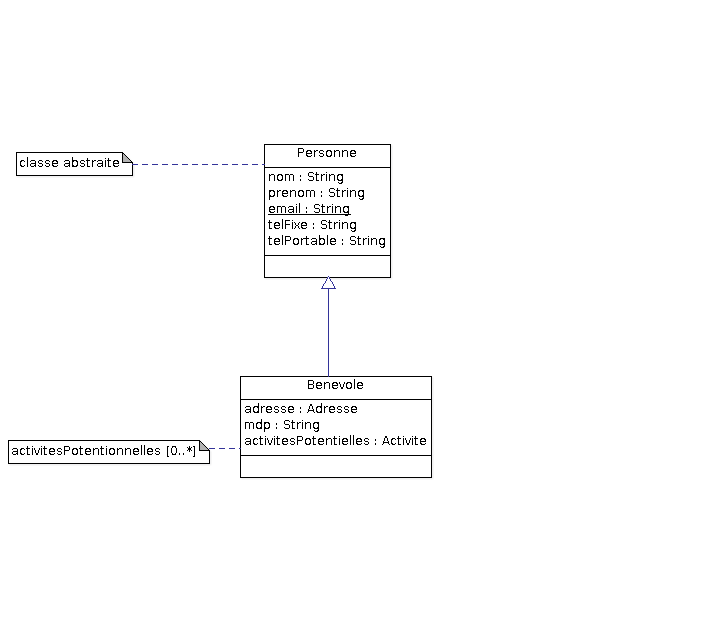
\includegraphics[scale=0.4]{images/classeBenevole.png}
	 \caption{Classe Benevole}
	 \label{classeBenevole}
\end{figure}

Les figures \ref{utilisateurNonConnecte} et \ref{utilisateurConnecte} présentent les diagrammes de cas d'utilisation propres aux actions possibles pour un utilisateur connecté et un utilisateur non connecté.\\
Les figures \ref{fonctionnalite1creationDUnUtilisateurs}, \ref{fonctionnalite1modificationDUnProfil}  et \ref{fonctionnalite1modificationDUnProfilAdmin} présentent respectivement la maquette de l'interface de création de profil et celles de la modification de profil (par un l'utilisateur puis par l'administrateur). \\
\begin{figure}[H]
	\centering
	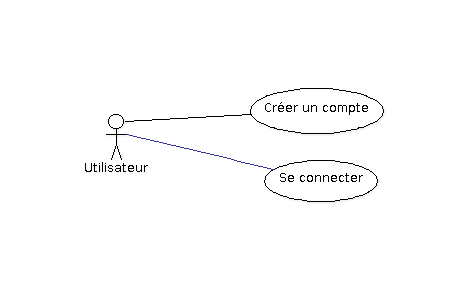
\includegraphics[scale=0.4]{images/casDUtilisation/fonctionnalite1UtilisateurNonConnecte.png}
	 \caption{Cas d'utilisation  d'un utilisateur non connecté}
	 \label{utilisateurNonConnecte}
\end{figure}

\begin{figure}[H]
	\centering
	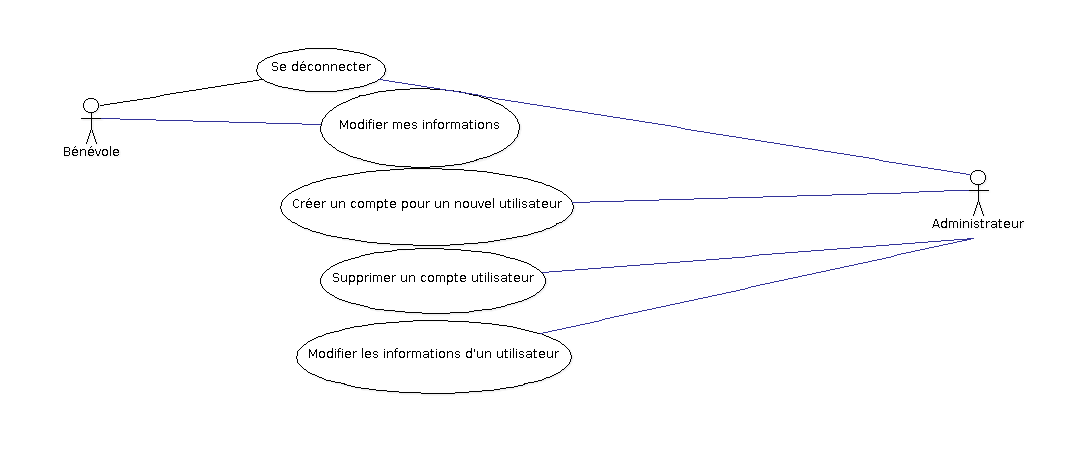
\includegraphics[scale=0.4]{images/casDUtilisation/fonctionnalite1UtilisateurConnecte.png}
	 \caption{Cas d'utilisation  d'un utilisateur connecté}
	 \label{utilisateurConnecte}

\end{figure}


% Figure : version 1.00, date 24/02/16, auteur Michel Cressant
\begin{figure}[H]
	\centering
	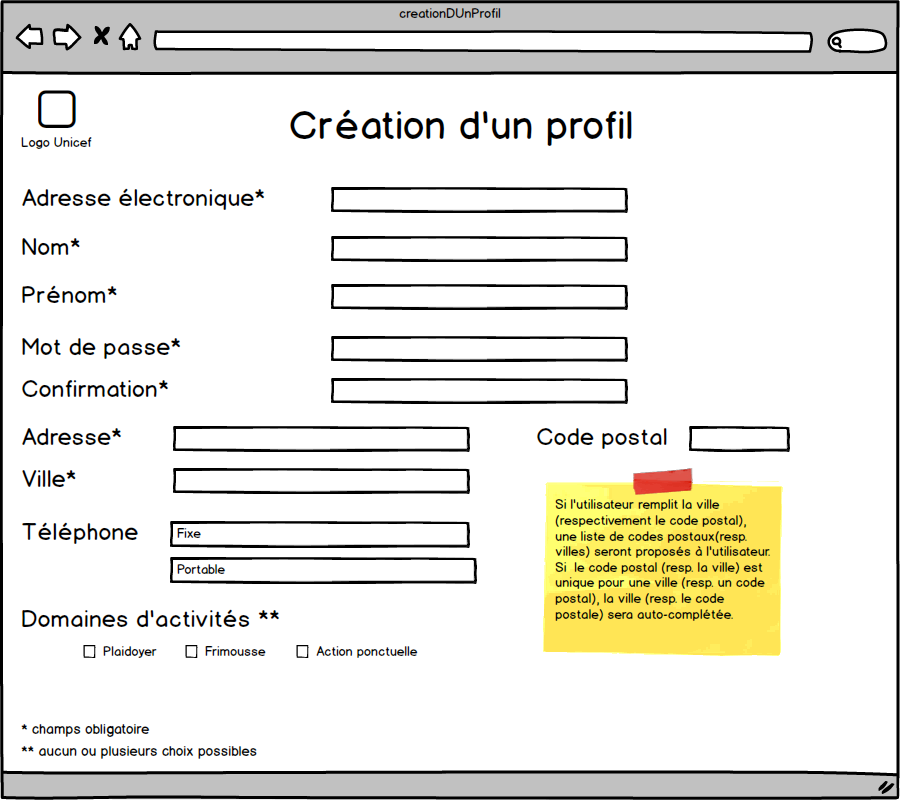
\includegraphics[scale=0.4]{images/maquettes/fonctionnalite1CreationDUnProfil.png}
	 \caption{Maquette~: Creation d'un utilisateur}
 \label{fonctionnalite1creationDUnUtilisateurs}
\end{figure}

% Figure : version 1.00, date 24/02/16, auteur Michel Cressant
\begin{figure}[H]
	\centering
	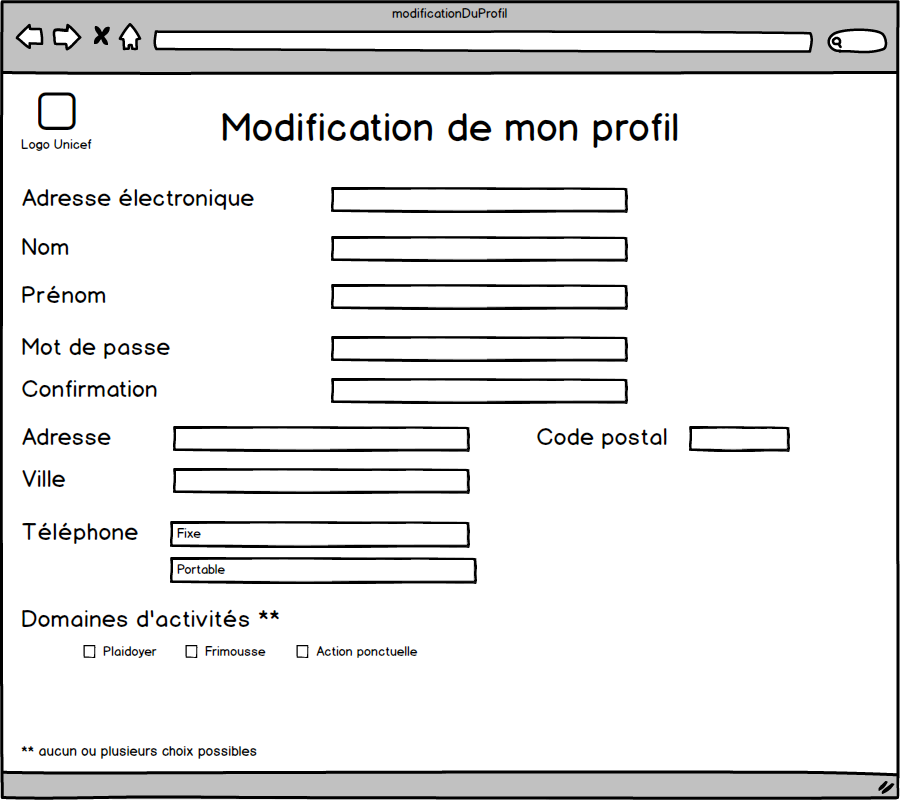
\includegraphics[scale=0.4]{images/maquettes/fonctionnalite1ModificationDUnProfil.png}
	 \caption{Maquette~: Modification des informations d'un utilisateur par l'utilisateur}
	 \label{fonctionnalite1modificationDUnProfil}
\end{figure}


% Figure : version 1.00, date 24/02/16, auteur Michel Cressant
\begin{figure}[H]
	\centering
	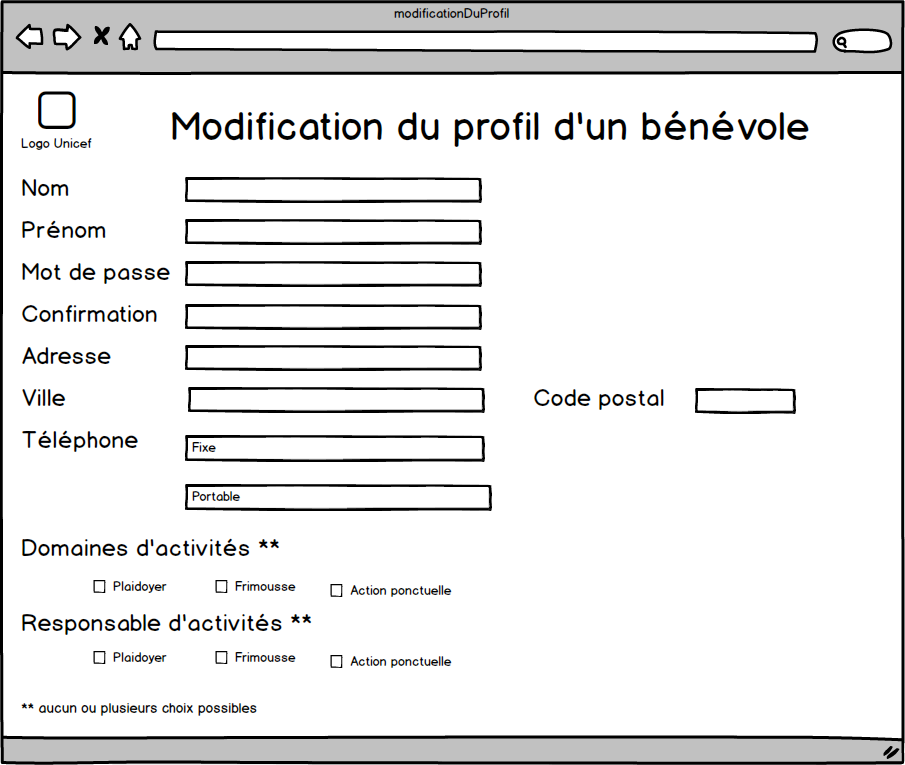
\includegraphics[scale=0.4]{images/maquettes/fonctionnalite1ModificationDUnProfilAdmin.png}
	 \caption{Maquette~: Modification des informations d'un utilisateur par l'administrateur}
	 \label{fonctionnalite1modificationDUnProfilAdmin}
\end{figure}

Un administrateur global est un utilisateur qui a tous les droits. \\ Un administrateur local est un responsable d'activité, il a des droits de lecture et de modification sur son activité. \\ Un bénévole a des droits de lecture et de modification sur ses informations personnelles et seulement des droits de lecture sur les informations concernant ses domaines d'activité. Il pourra également s'attribuer une activité, entrer et modifier des informations sur cette activité.\\
Il pourra exister plusieurs administrateurs globaux, plusieurs administrateurs locaux et plusieurs bénévoles. Un administrateur local peut être responsable de plusieurs activités.



Les activités potentielles pourront ainsi avoir plusieurs responsables et seront composées des actions ponctuelles, des plaidoyers et des actions frimousses. \\

Un ou plusieurs utilisateurs peuvent être responsable d'un, plusieurs ou aucun projets (école, lycéen ou étudiant).\\

La création et la modification d'une caractéristique concernant un bénévole devront faire l'objet d'un envoi de mail au bénévole l'informant de la création ou modification voulue et donnant l'ensemble des informations le concernant. Un an après une modification sur une caractéristique sur un utilisateur, l'ancienne caractéristique sera supprimée. \\


Une contrainte d'intégrité du système est que toute action effectuée doit avoir été réalisée par un bénévole existant. \\
Si le nom de l'intervenant ayant effectué une action n'est pas connu, l'action sera attribuée a un bénévole spécial. Une fonction d'interrogation permettant de donner la liste des interventions effectuées par ce bénévole fictif sera implémentée afin d'engager les actions nécessaires pour trouver le nom du bénévole ayant effectué cette action. \\


La procédure de connexion au système sera basée sur le couple login (adresse e-mail) / mot de passe.


% version 1.00, date 23/02/16, auteur Matthieu Martins-Baltar
\subsection{Fonctionnalité 2}
La fonctionnalité 2 du système devra permettre les opérations conventionnelles de gestion individuelle comme la création d'un établissement dans le système, la modification des
caractéristiques le concernant, la suppression d'un établissement. La figure \ref{creationDunEtablissement} présentera le diagramme de cas d'utilisation concernant la création d'un établissement.\\
 Comme pour un bénévole, la suppression devra être logique et non physique de façon à ne pas perdre l'historique des actions effectuées dans cet établissement sachant que la disparition peut être temporaire en fonction de l'ouverture et la fermeture de classes. \\

\begin{figure}[H]
	\centering
	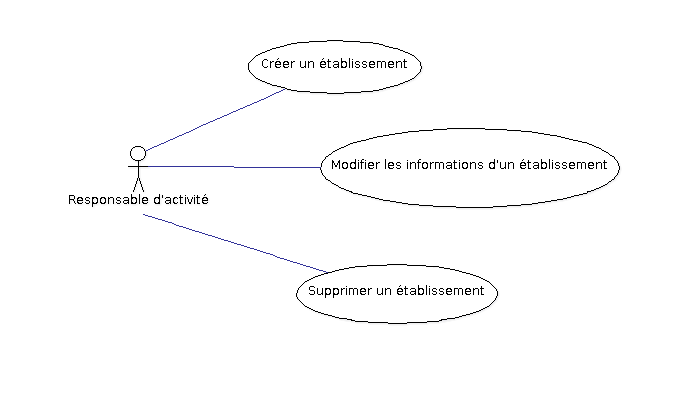
\includegraphics[scale=0.4]{images/casDUtilisation/fonctionnalite2Etablissement.png}
	 \caption{Cas d'utilisation~: créer un établissement}
	 \label{creationDunEtablissement}
\end{figure}


Les informations associées à un établissement sont :
\begin{itemize}
\item sa ville de rattachement (unique), 
\item son nom lorsqu'il existe (attention dans la même ville il peut y avoir une école élémentaire et une école maternelle sans nom spécifique), 
\item son adresse,
\item son code postal,
\item le responsable de l'établissement, 
\item le contact plaidoyers (facultatif),
\item le contact frimousse (facultatif),
\item le contact pour les activités ponctuelles (facultatif),
\item le numéro de téléphone fixe de l'établissement, 
\item la ou les adresse(s) électronique(s) de l'établissement (attention toutes les adresses électroniques ne sont pas forcément celles définies par le rectorat notamment pour les établissements privés ou pour les centres de loisirs), 
\item le nom, le numéro de téléphone fixe et/ou portable de l'enseignant demandant une intervention, son adresse électronique (toutes ces informations ne sont pas forcément disponibles). Il peut y avoir plusieurs enseignants pour la même classe (donc plusieurs contacts possibles).
\item sa localisation géographique (Latitude-Longitude en WGS84) si elle est disponible.
\item son type (enseignement ou centre de loisirs)
\\
\end{itemize}
Les enseignements ont un UAI et un type d'enseignement (l'enseignement supérieur, les lycées, les collèges, les écoles élémentaires et maternelles). \\
Les centres de loisirs ont un type de centre (maternelle, élémentaire et adolescent). 


\newpage
\subsection{Fonctionnalité 3}
La fonctionnalité 3 permettra l'envoi de courriers électroniques aux établissements qui contiendront une lettre type accompagnée d'une plaquette en pièce jointe.La figure \ref{envoiMailsCibles} présentera le diagramme de cas d'utilisation concernant l'envoi d'emails ciblés aux établissements.\\
 La plaquette sera fonction du type d'établissement et envoyé au format pdf. Le corps de l'e-mail contiendra la lettre type. La figure \ref{fonctionnalite3MailType} présentera une maquette du courriel type envoyé aux établissements.\\


\begin{figure}[H]
	\centering
	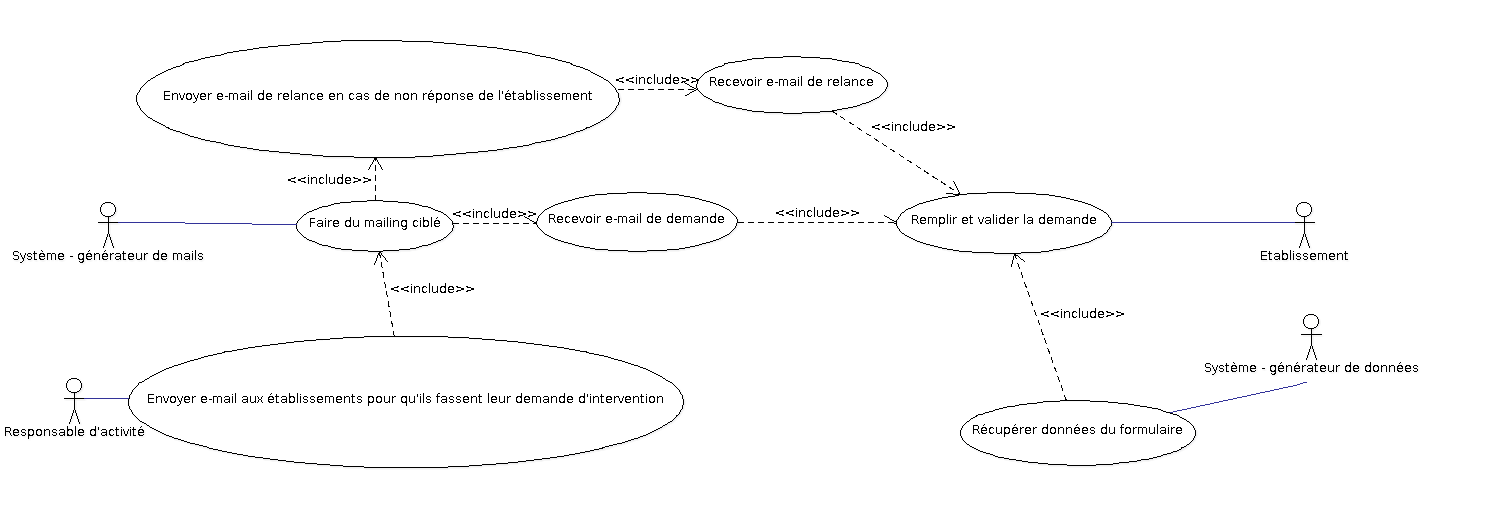
\includegraphics[scale=0.4]{images/casDUtilisation/fonctionnalite3Mailing.png}
	 \caption{Cas d'utilisation~: Envoyer des e-mails ciblés}
	 \label{envoiMailsCibles}
\end{figure}

% Figure : version 1.00, date 24/02/16, auteur Michel Cressant
\begin{figure}[H]
	\centering
	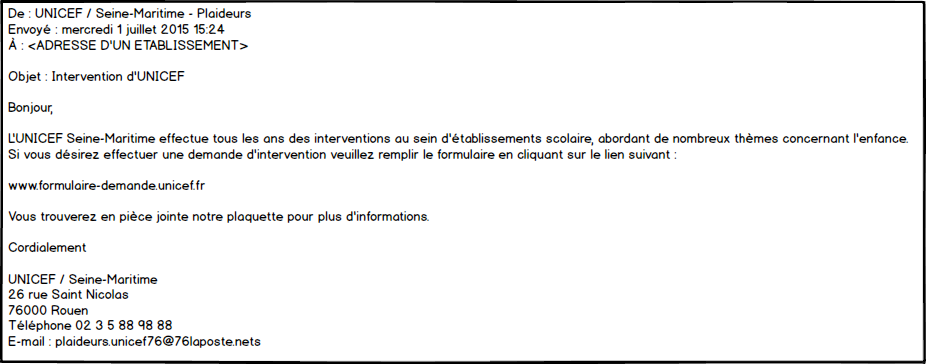
\includegraphics[scale=0.57]{images/maquettes/fonctionnalite3MailType}
	\caption{Maquette~: Email type envoyé aux établissement}
	\label{fonctionnalite3MailType}
\end{figure}


Cette fonctionnalité doit également permettre un envoi ciblé en fonction de plusieurs critères qui pourront être sélectionnés simultanément :
\begin{itemize}
\item le type de l'établissement (maternelle, élémentaire, centre de loisirs,...), 
\item la distance des villes suivantes : Rouen, Le Havre, Yvetot, Fécamp, Dieppe et Neuchâtel en Bray à la ville de l'établissement,
\item la non-réponse à une précédente sollicitation pour cette année scolaire (un mail de relance),
\item la réponse à une précédente sollicitation pour cette année scolaire (les établissements ayant demandé une action de frimousses ou une action ponctuelle mais pas de plaidoyer),
\item un sous-ensemble spécifique des adresses obtenues soit manuellement soit par l'application d'un critère (les écoles d'une ville donnée, un type donné par exemple),
\item exclure de la liste les établissements ayant fait une demande qui n'a pas pu être satisfaite par les plaideurs (pour des raisons d'emploi du temps, distance, ...). \\
\end{itemize}

Chaque e-mail invitera l'établissement à se connecter à un lien (actif) contenant un formulaire à remplir pour effectuer une demande d'intervention. Les champs à remplir seront : 
\begin{itemize}
\item la ville de l'établissement, 
\item le nom de l'établissement, 
\item le nom de la personne référente sur cette action, 
\item l'adresse électronique de la personne référente sur cette action ou celle de l'établissement si la personne  référente n'en a pas, 
\item le numéro de téléphone de la personne référente ou de l'établissement si la personne référente n'en a pas,
\item les plages de dates souhaitées pour l'intervention (date de début et date de fin),
\item les disponibilités (jours et les moments souhaités comme dans le formulaire actuel), 
\item le matériel disponible (vidéo projecteur, TBI, enceinte ou  aucun), 
\item le type de classes concernées (maternelle, élémentaire (ou centre de loisirs élémenaire), collège (ou centre de loisirs collège), lycée, enseignement supérieur)
\item le niveau de la classe, 
\item le thème dominant de l'intervention souhaité, 
\item le nombre d'élèves à préciser si plusieurs classes,
\item des remarques.
\end{itemize}
La figure \ref{fonctionnalite3FormulaireDeDemandeDInterventions} présentera une maquette du formulaire de demande d'intervention.
\newpage
% Figure : version 1.00, date 24/02/16, auteur Michel Cressant
\begin{figure}[H]
	\centering
	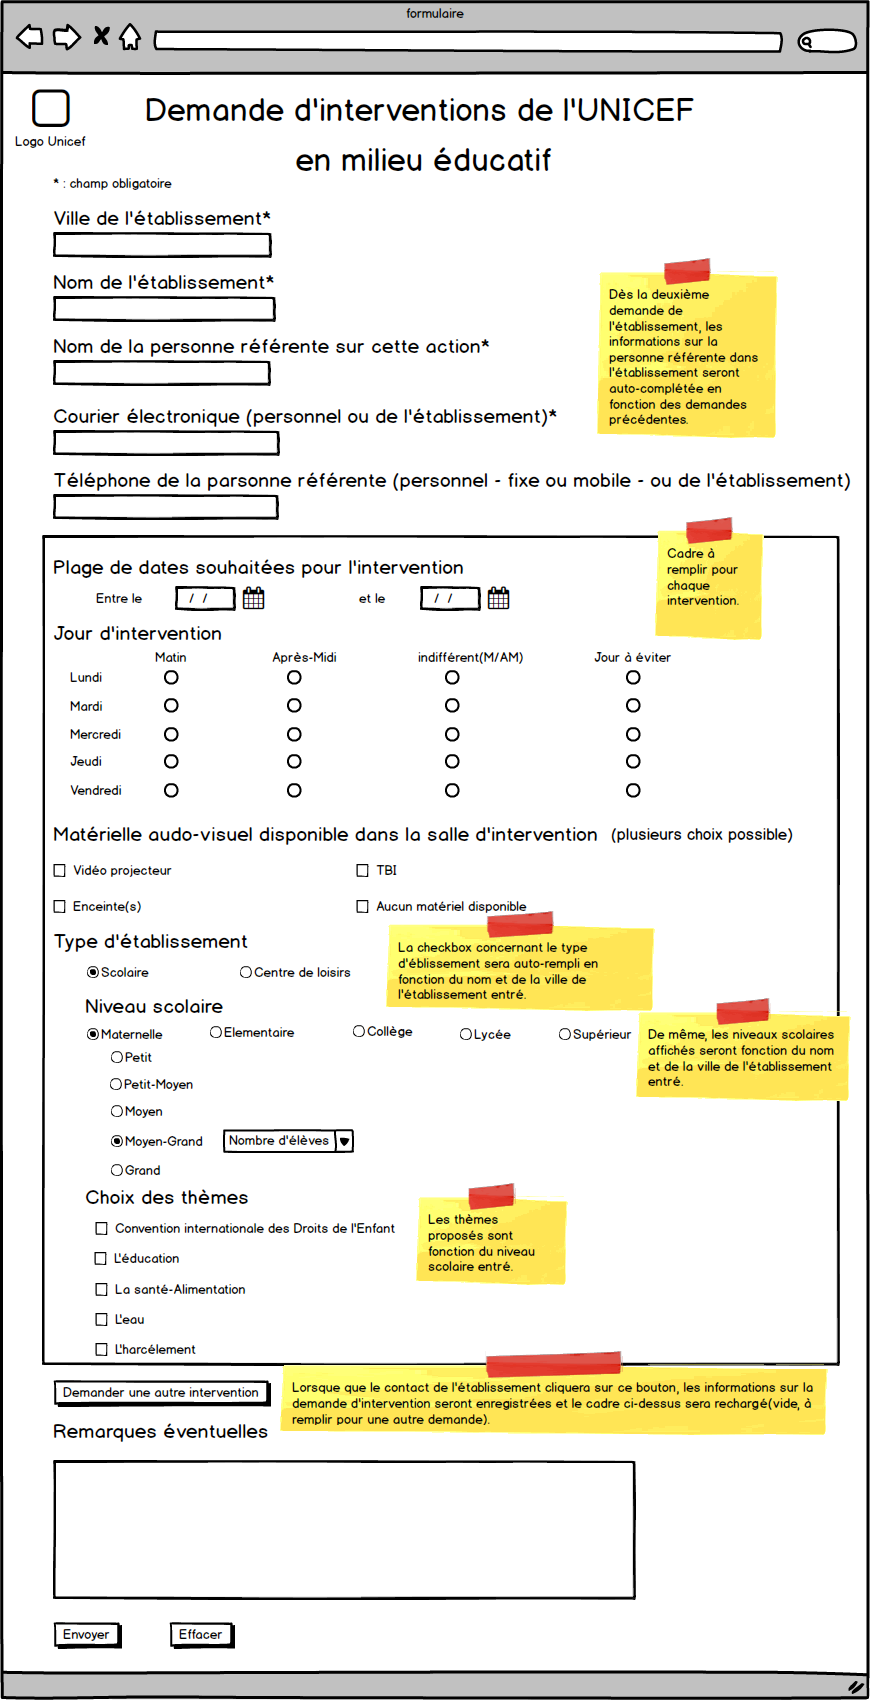
\includegraphics[scale=0.415]{images/maquettes/fonctionnalite3FormulaireDeDemandeDInterventions.png}
	\caption{Maquette~: Formulaire de demande d'intervention}
	\label{fonctionnalite3FormulaireDeDemandeDInterventions}
\end{figure}

Les réponses à ce formulaire viendront alimenter la base de données des demandes d'intervention. \\
Concernant le matériel disponible , plusieurs matériels pourront être choisis. \\
Concernant le niveau de la classe, nous reprendrons ceux proposés dans le formulaire actuel. Si la classe regroupe le niveau Grande Section et CP, l'information doit être précisée en remarque.
Concernant les classes spéciales (classe pour l'inclusion scolaire, sections d'enseignement général et professionnel adapté, etc...), elles ne seront pas traitées comme les classes par défaut, elles seront précisées dans le champs remarque.
\\
Les thèmes des interventions ne seront pas prédéfinis pour les lycées et l'enseignement supérieur. Ceux-ci seront renseignés dans un champs texte par l'établissement demandeur. Pour les autres types d'établissement, nous reprendrons les thèmes du formulaire actuel.

% version 1.00, date 23/02/16, auteur Matthieu Martins-Baltar
\newpage
\subsection{Fonctionnalité 4}
La fonctionnalité 4 consiste en premier lieu à faciliter le remplissage du formulaire par l'établissement. 
Une complétion automatique du nom de la ville, de l'établissement, des niveaux scolaires devra être mise en place. Cependant, il n'y en aura pas pour les informations personnelles du demandeur (comme  par exemple son numéro de téléphone ou son adresse électronique).\\
La figure \ref{recevoirDemandesDIntervention} présentera un diagramme de cas d'utilisation présentant la réception de demande d'intervention d'un établissement.\\
Les données personnelles concernant les contacts dans l'établissement seront seulement un complément des informations disponibles pour un établissement. Elles pourront être mises à jour chaque année dans différents cas comme par exemple lors d'une mutation ou d'un départ en retraite ou encore d'un nouvel enseignant.   \\

La fonctionnalité 4 permettra également l'envoi d'un e-mail de confirmation à l'établissement lorsque ce dernier aura rempli et validé le formulaire. Cet e-mail proposera également à l'établissement d'annuler la demande d'intervention. \\ Une copie de cet e-mail sera adressée au responsable local de chaque activité.
La figure \ref{maquetteCourrielConfirmation} présentera une maquette de l'e-mail de confirmation de l'établissement.\\
\begin{figure}[H]
	\centering
	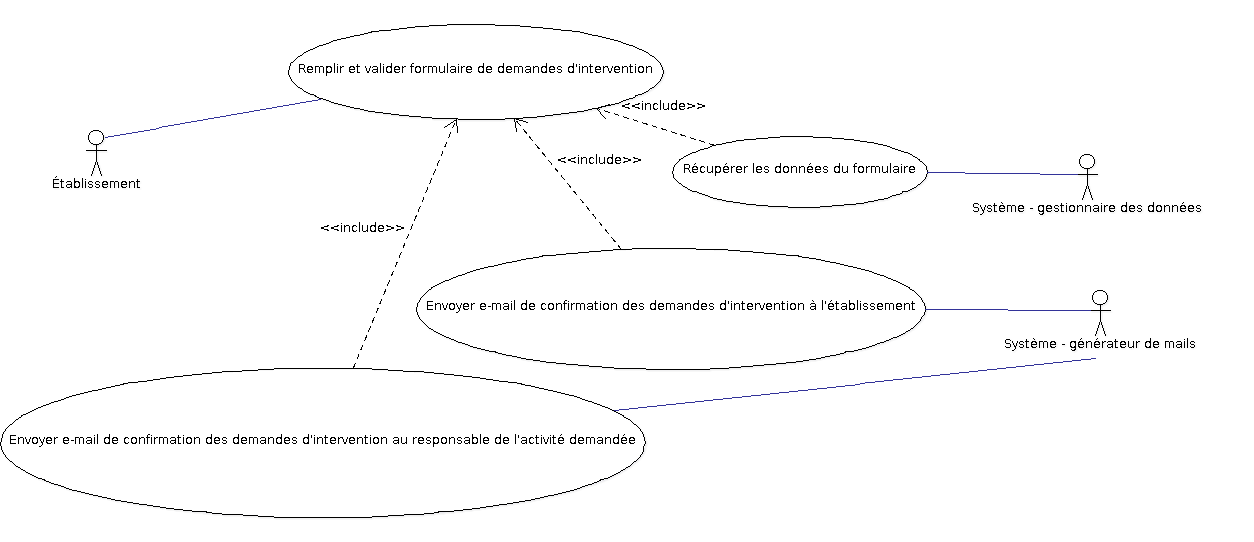
\includegraphics[scale=0.4]{images/casDUtilisation/fonctionnalite4ReceptionIntervention.png}
	 \caption{Cas d'utilisation~: Recevoir la demande d'intervention d'un établissement}
	 \label{recevoirDemandesDIntervention}
\end{figure}

% Figure : version 1.00, date 24/02/16, auteur Michel Cressant
\begin{figure}[H]
	\centering
	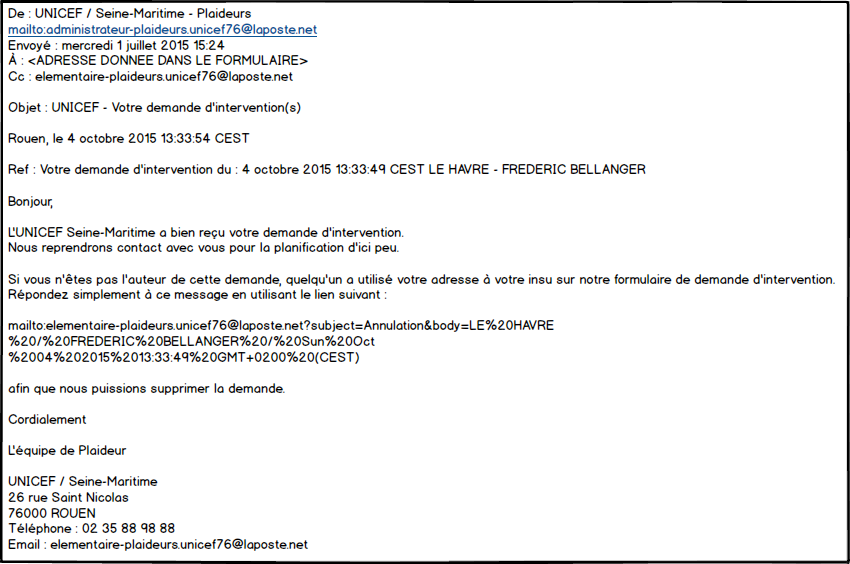
\includegraphics[scale=0.615]{images/maquettes/fonctionnalite4MailConfirmationReceptionDemande.png}
	\caption{Maquette~: Email de confirmation de reception d'une demande d'une école élémentaire}
	\label{maquetteCourrielConfirmation}
\end{figure}

Si un établissement annule une demande d'intervention (grâce à l'e-mail de confirmation d'une demande d'intervention), une procédure supprimera cette demande et enverra des e-mails de confirmation de suppression de cette demande au responsable de l'activité initialement demandée et à l'établissement.Les figures \ref{maquetteCourrielConfirmationAnnulationEtablissement} et {maquetteCourrielConfirmationAnnulationResponsable} présentent une maquette de l'e-mail de confirmation d'annulation pour un établissement et pour un responsable d'activité.\\
  


% Figure : version 1.00, date 24/02/16, auteur Michel Cressant
\begin{figure}[H]
	\centering
	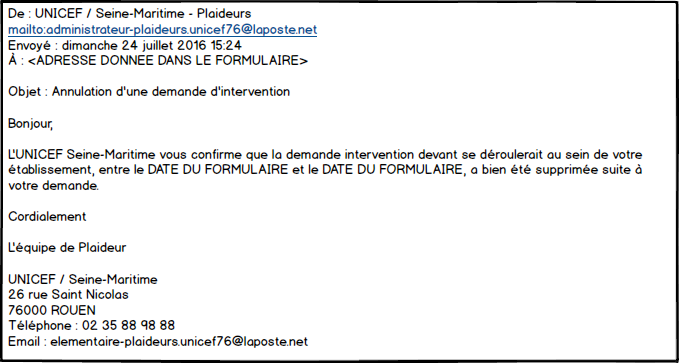
\includegraphics[scale=0.7]{images/maquettes/fonctionnalite4MailConfirmationSuppressionDemandePourEtablissement.png}
	\caption{Maquette~: Email de confirmation d'annulation d'une intervention pour un établissement}
	\label{maquetteCourrielConfirmationAnnulationEtablissement}
\end{figure}

% Figure : version 1.00, date 24/02/16, auteur Michel Cressant
\begin{figure}[H]
	\centering
	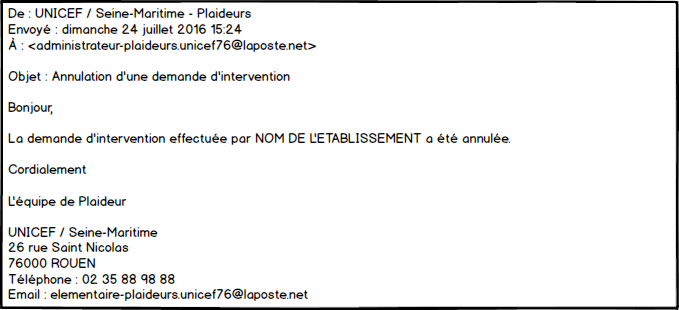
\includegraphics[scale=0.7]{images/maquettes/fonctionnalite4MailConfirmationSuppressionDemandePourAdmin.png}
	\caption{Maquette~: Email de confirmation d'annulation d'une intervention pour le responsable d'activité}	\label{maquetteCourrielConfirmationAnnulationResponsable}
\end{figure}

\subsection{Fonctionnalité 5}
La fonctionnalité 5 permettra d'afficher une carte montrant les lieux où des demandes d'intervention ont été faites pour un créneau que l'utilisateur aura entré.
La figure \ref{maquetteCarteIntervention} présente une maquette de la carte des interventions.

% Figure : version 1.00, date 24/02/16, auteur Mélissa Bignoux
\begin{figure}[H]
	\centering
	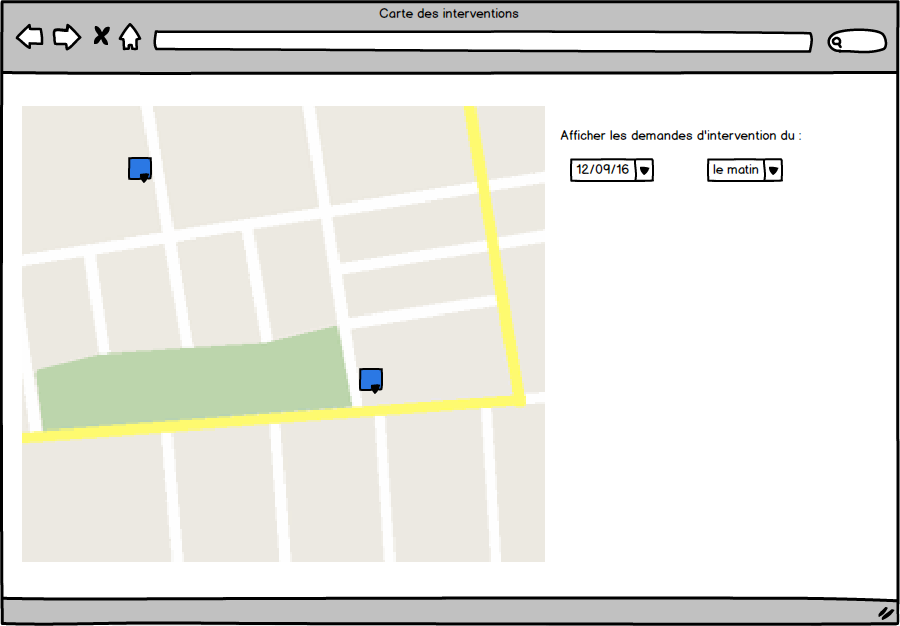
\includegraphics[scale=0.575]{images/maquettes/fonctionnalite5CarteDesInterventions.png}
	\caption{Maquette~: Carte des interventions en fonction d'une date choisie et du moment de la journée}
	\label{maquetteCarteIntervention}
\end{figure}

La fonctionnalité 5 consistera également à planifier les interventions c'est-à-dire qu'un plaideur s'attribue une intervention.
Lors de chaque affectation, un e-mail d'information de prise en charge de la demande par l'équipe de plaideur sera envoyé à l'établissement demandeur ainsi qu'au responsable de l'activité demandée.
La figure \ref{courrielPrisCharge} présente la maquette de cet email d'information de prise en charge. 
Une intervention ne peut être attribuée qu'à un utilisateur.
  La figure \ref{visualiserESAttribuer} présente le diagramme de cas d'utilisation sur la visualisation et l'attribution des interventions.

\\

\begin{figure}[H]
	\centering
	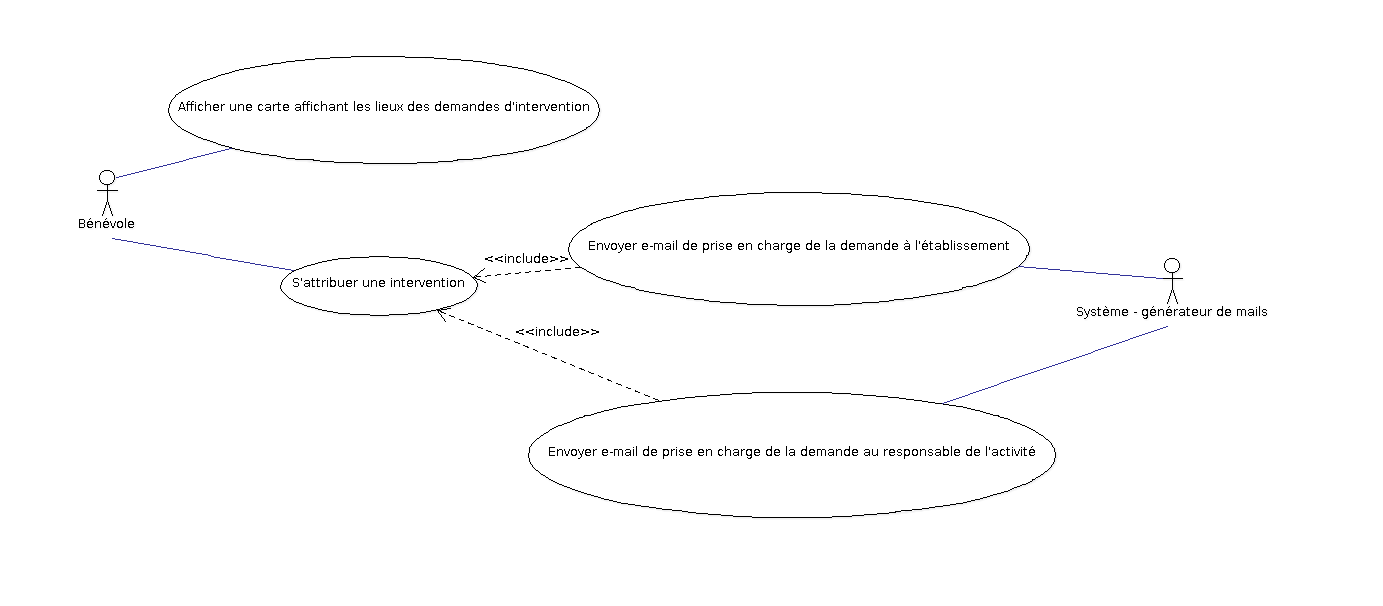
\includegraphics[scale=0.4]{images/casDUtilisation/fonctionnalite5Attribution.png}
	 \caption{Cas d'utilisation~: Visualiser les demandes et s'attribuer des interventions}
	 \label{visualiserESAttribuer}
\end{figure}

% Figure : version 1.00, date 24/02/16, auteur Michel Cressant
\begin{figure}[H]
	\centering
	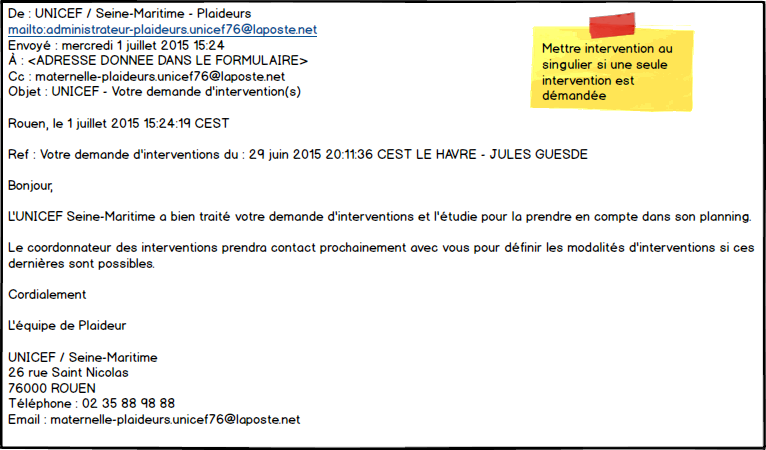
\includegraphics[scale=0.675]{images/maquettes/fonctionnalite5MailDePriseEnCharge.png}
	\caption{Maquette~: Email de prise en charge d'une intervention}
	\label{courrielPrisCharge}
\end{figure}


\subsection{Fonctionnalité 6}
Une fois que le plaideur a défini une date pour son intervention (suite à échange de courriers électroniques avec le contact de l'établissement), il met à jour les informations concernant l'intervention (date, heure, nombre d'élèves, ...). Le demandeur reçoit alors un mail de confirmation l'informant du jour de l'heure et du lieu de l'intervention avec le nom et les coordonnées (adresse électronique, téléphone) du plaideur. Le texte de ce message est à définir et à faire valider par le responsable des plaideurs. Cette procédure est décrite sur la figure \ref{diagrammeSequenceMiseAJourIntervention} : 
\begin{figure}[H]
	\centering
	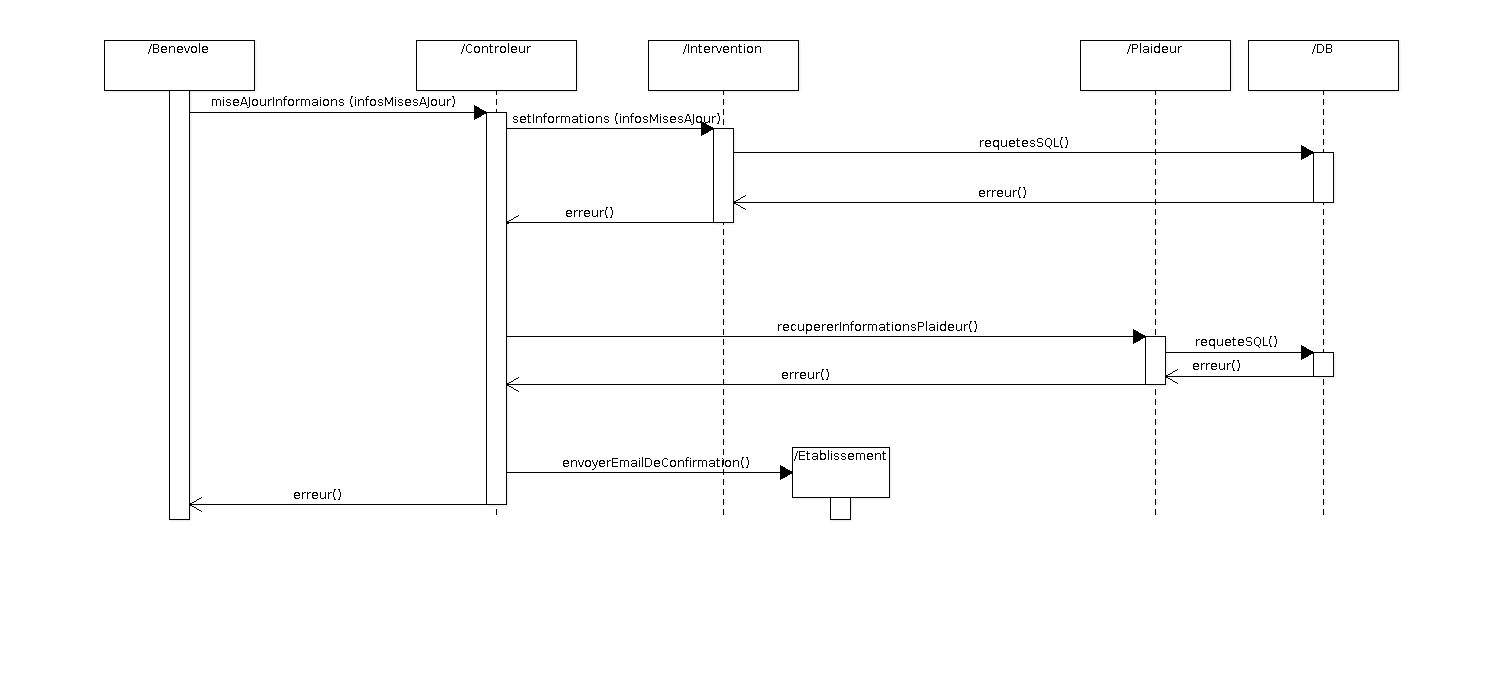
\includegraphics[scale=0.35]{images/diagrammeSequence}
	 \caption{Diagramme de séquence~: Mise à jour d'intervention}
	 \label{diagrammeSequenceMiseAJourIntervention}
\end{figure}

  La figure \ref{mettreAJourInterventions} présente le diagramme de cas d'utilisation de la mise à jour d'information relative à une intervention. La figure \ref{courrielRecapitulatifIntervention} présente la maquette de l'email récapitulatif des informations concernant l'intervention. 
 
\begin{figure}[H]
	\centering
	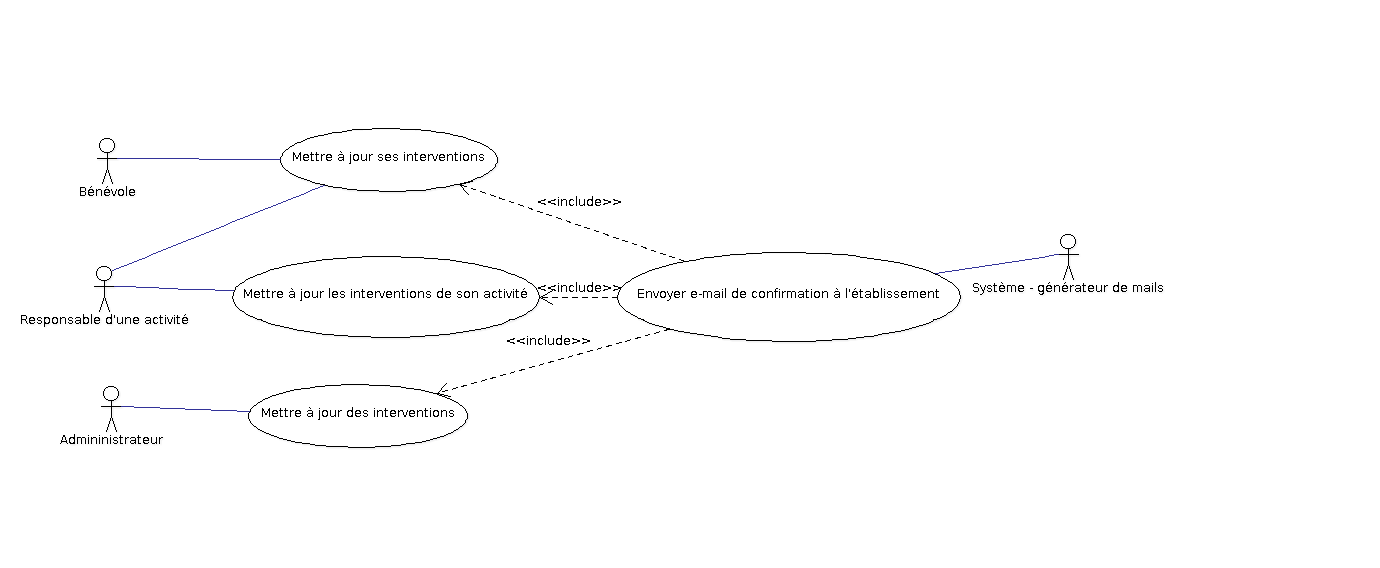
\includegraphics[scale=0.4]{images/casDUtilisation/fonctionnalite6MiseAJourIntervention.png}
	 \caption{Cas d'utilisation~: mettre à jour les informations d'interventions}
	 \label{mettreAJourInterventions}
\end{figure}


% Figure : version 1.00, date 24/02/16, auteur Mélissa Bignoux
\begin{figure}[H]
	\centering
	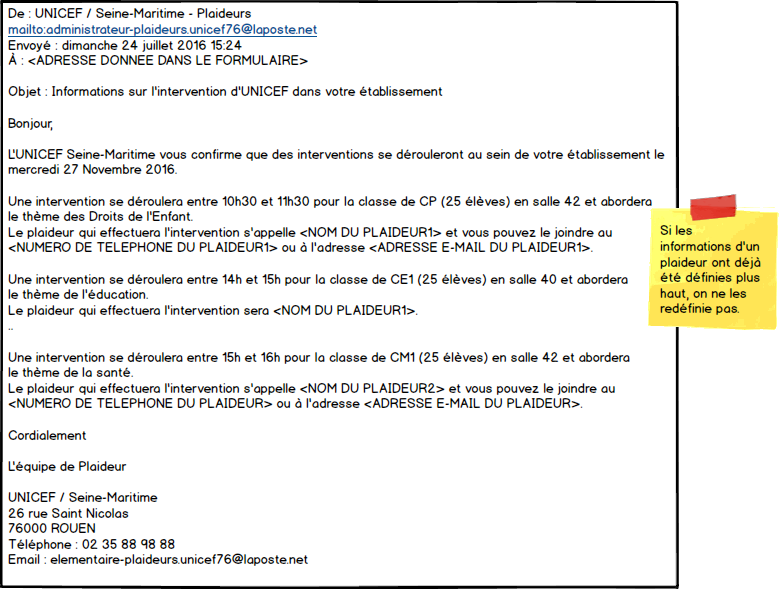
\includegraphics[scale=0.7]{images/maquettes/fonctionnalite6MailDInformationPourLEtablissement.png}
	\caption{Maquette~: Email récapitulatif des informations concernant l'intervention}
	\label{courrielRecapitulatifIntervention}
\end{figure}


% version 1.00, date 23/02/16, auteur Matthieu Martins-Baltar
\newpage
\subsection{Fonctionnalité 7}
La fonctionnalité 7 permettra d'envoyer un e-mail de rappel à l'établissement et au contact dans l'établissement (si son adresse électronique est différente de celle de l'établissement), une semaine avant l'intervention. Le texte de ce message sera à définir avec \nomClient{} et à faire valider par le responsable des plaideurs. La maquette de cet email est présenté dans la figure \ref{courrielRappelEtablissement}. \\

% Figure : version 1.00, date 24/02/16, auteur Michel Cressant
\begin{figure}[H]
	\centering
	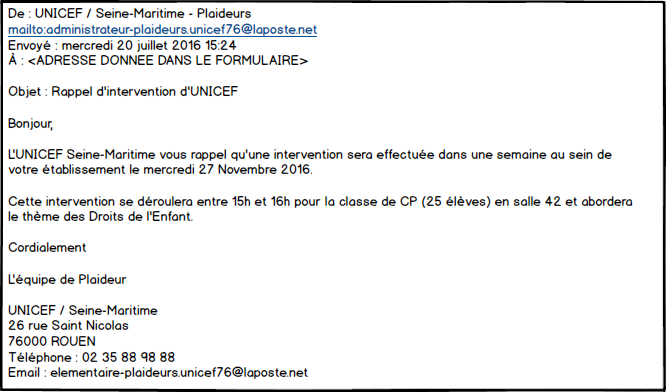
\includegraphics[scale=0.675]{images/maquettes/fonctionnalite7MailDeRappelPourLEtablissement.png}
	\caption{Maquette~: Email de rappel d'intervention pour un établissement}
	\label{courrielRappelEtablissement}
\end{figure}

Trois jours avant l'intervention, le plaideur recevra un e-mail de rappel avec les informations associées (date, heure, lieu, thème, nombre d'élèves, remarques, niveau des élèves). 
La maquette de cet email est présenté dans la figure \ref{courrielRappelPlaideur}. \\
\\

% Figure : version 1.00, date 24/02/16, auteur Michel Cressant
\begin{figure}[H]
	\centering
	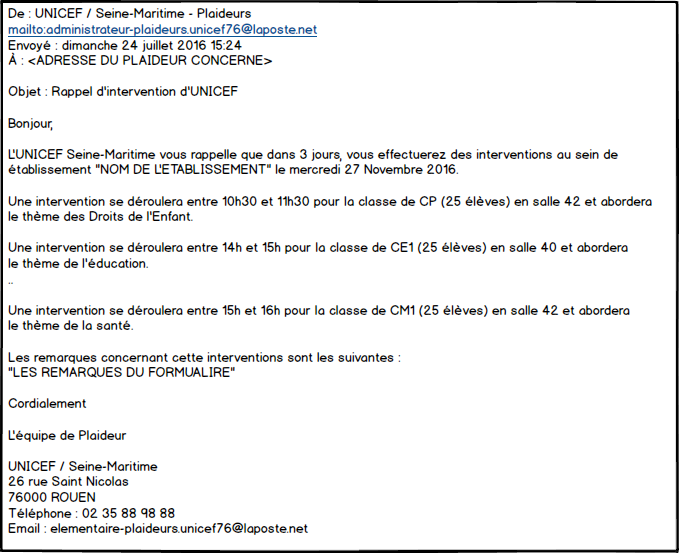
\includegraphics[scale=0.65]{images/maquettes/fonctionnalite7MailDeRappelPourLePlaideur.png}
	\caption{Maquette~: Email de rappel d'intervention pour le plaideur}
	\label{courrielRappelPlaideur}
\end{figure}

La figure \ref{envoiRappel} présente le diagramme de cas d'utilisation concernant l'envoi d'email de rappel.
 
\begin{figure}[H]
	\centering
	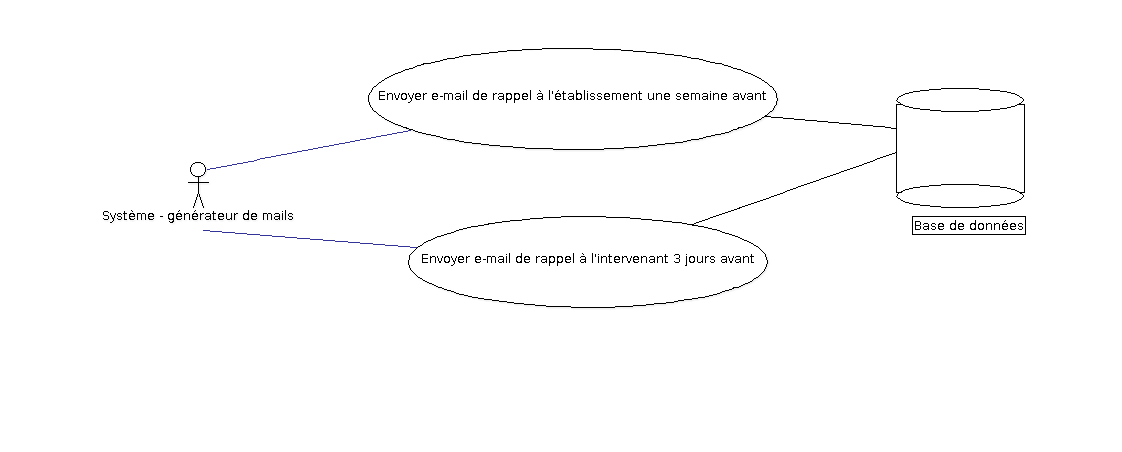
\includegraphics[scale=0.4]{images/casDUtilisation/fonctionnalite7Rappels.png}
	 \caption{Cas d'utilisation~: Envoyer des emails de rappels}
	 \label{envoiRappel}
\end{figure}


% version 1.00, date 23/02/16, auteur Matthieu Martins-Baltar
\subsection{Contraintes Produits}
Dans cette sous-partie, nous allons décrire les contraintes produits, c'est-à-dire des contraintes ayant trait au système à proprement parler.\\

L'interface de l'application se présentera sous la forme d'une page web qui sera visualisée à partir d'un navigateur. Les navigateurs principaux, Chrome, Firefox, Safari doivent être compatibles et capables d'afficher correctement la page. L'équipe \PIC{} devra spécifier au client les versions de navigateur compatible avec l'application.  Le code de cette page devra répondre aux normes de la W3C. De plus, l'interface devra être \emph{responsive} et utilisable depuis un smartphone. Enfin, le design de l'interface doit permettre une utilisation simple à un utilisateur inexpérimenté.\\

La partie serveur de l'application devra être légère et pouvoir fonctionner sur un serveur de faible dimension.\\

 
% version 1.00, date 23/02/16, auteur Matthieu Martins-Baltar
\subsection{Contraintes de Réalisation}
Dans cette sous-partie, nous allons lister les contraintes de réalisation, telles que les demandes de documentation ou des contraintes de langage.\\

Il n'y a aucune contrainte de langage de programmation, mais il est à noter qu'il doit s'agir de langages adaptés aux technologies web. Par exemple la partie frontend de notre application ne pourra être qu'en Javascript.\\

La base de donnée utilisera PostgreSQL et PostGIS afin d'intégrer de manière optimale le service OpenStreetMap.\\

Il est demandé une documentation technique à tous les niveaux du projet. Tout d'abord une documentation conceptuelle, une documentation des packages, une documentation détaillée, ainsi que des tests unitaires détaillés et documentés. Cette documentation doit permettre à une future équipe de développement de retravailler sur le projet sans difficulté. Doivent également être documentées, les règles de programmation, les conventions de nommage et les instructions permettant l'installation du logiciel.\\

Enfin, une documentation utilisateur, accompagnée d'une foire aux questions accessible à tous les utilisateurs sera livrée avec le lot2.






\begin{appendix}
\part*{Annexes}
\addcontentsline{toc}{part}{Annexes}

\listoffigures
\addcontentsline{toc}{chapter}{Table des figures}
	 
\listoftables
\addcontentsline{toc}{chapter}{Liste des tableaux}
\end{appendix}
\pageQuatriemeCouverture

\end{document}
